%\chapter{Введение}				% Заголовок
%\addcontentsline{toc}{section}{Введение}	% Добавляем его в оглавление

\section{Классическая криптография}
Задача передачи секретной информации известна человечеству с самых ранних времён. Из основных типов сведений, для которых может быть важна их
секретная передача, можно выделить следующие:
\begin{itemize}
  \item важная государственная информация,
  \item информация, содержащая военные секреты,
  \item коммерческие данные,
  \item личная конфиденциальная информация.
\end{itemize}

Исход большого количества военных кампаний и финансовый успех многих корпораций всегда был напрямую связан в том числе с умением передавать
информацию без её утечки к третьим лицам, что говорит о существенной ценности развития технологий секретной передачи данных.

Традиционно для шифрования информации используются два подхода: симметричные криптосистемы и асимметричные.
В симметричных методах шифрования применяется один и тот же ключ как для шифрования, так и для расшифрования данных. Обе стороны коммуникации должны знать этот ключ и хранить его в секрете.
При асимметричном шифровании используется два ключа: открытый и закрытый. Открытый ключ передаётся по незащищённому каналу и используется для проверки электронной подписи и шифрования сообщения.
Закрытый ключ используется для расшифрования сообщений и генерации электронной подписи. 

Асимметричные криптосистемы имеют ряд преимуществ перед симметричными: 
\begin{itemize}
  \item не нужно предварительно передавать секретный ключ по надёжному каналу,
  \item этот секретный ключ известен только одной стороне, 
  \item пару ключей можно долгое время не менять.
\end{itemize}

Однако есть и серьезные недостатки, которые не позволяют полностью перейти на использование асимметричных систем: 
\begin{itemize}
  \item в алгоритм сложно внести изменения, 
  \item ключи имеют большую длину,
  \item по сравнению с симметричными криптосистемами процесс шифрования и расшифрования медленнее на порядки, 
  \item требуются значительно большие вычислительные мощности для функционирования асиметричной криптосистемы. 
\end{itemize}

Для симметричных криптосистем была доказана абсолютная криптостойкость\cite{vernam_security_proof}, в то время как разработка квантовых компьютеров полностью разрушит асимметричные схемы шифрования. Остается одна проблема: как передать секретный ключ для симметричного шифрования. В классической физике этот вопрос не решается. Однако квантовая теория способна предложить некоторые решения.

\section{Основные результаты, важные для квантовой криптографии}

\subsection{Коллапс волновой функции}
Важным законом квантовой механики является коллапс волновой функции, или редукция. Это свойство означает переход состояния после измерения в одно из собственных состояний оператора измерения. Так, при измерении $\{M_i\}$ и получении результата $i$ исходное состояние будет преобразовано в 
\begin{equation} \rho'_i = \frac{\sqrt{M_i} \rho \sqrt{M_i}}{\tr M_i \rho}. \end{equation}

Это одно из важнейших для квантовой криптографии свойств, поскольку оно говорит о том, что попытки измерить систему ведут к помехам. Из этого следует, что попытки перехвата информации всегда можно детектировать по ошибкам на приёмной стороне.

\subsection{Невозможность достоверного различения неортогональных состояний}\label{no_discrimination_theorem}
Невозможность достоверного различения неортогональных квантовых состояний \cite{non_orthogonal_states_discrimination_theorem}~--- важный результат, на котором также во многом основывается секретность протоколов квантовой криптографии.

Этот результат можно сформулировать следующим образом: для чистых состояний \state{\psi_0} и \state{\psi_1} таких, что
$\scalar{\psi_0}{\psi_1} = \cos \alpha \neq 0$, не существует измерения $\{M_0, M_1\}$, которое давало бы точный результат, то есть соответствовало бы условиям
\begin{eqnarray}\label{measurement_operators_conditions}
  \conjstate{\psi_0} M_0 \state{\psi_0} = 1,\quad \conjstate{\psi_1} M_0 \state{\psi_1} = 0, \nonumber\\
  \conjstate{\psi_0} M_1 \state{\psi_0} = 0,\quad \conjstate{\psi_1} M_1 \state{\psi_1} = 1.
\end{eqnarray}

\subsection{Чёткие и нечёткие наблюдаемые}
Обычно под наблюдаемой подразумевают только ортогональное разложение единицы. Такие наблюдаемые будем называть \textit{чёткими наблюдаемыми}\cite{holevo}. В то же время требование взаимной ортогональности всех операторов не является обязательным, а в некоторых случаях выгоднее пользоваться наблюдаемыми, в которых не все операторы ортогональны друг другу, в целях получения максимального количества информации. Такие наблюдаемые называются \textit{нечёткими}.

На первый взгляд нечёткие наблюдаемые просто смешивают вероятности разных исходов и не могут принести дополнительной пользы. Однако это не так.
Рассмотрим пример, как нечёткая наблюдаемая может помочь различить неортогональные состояния \state{\varphi} и \state{\psi}: $ \scalar{\varphi}{\psi} = \cos \eta \neq 0.$

Одно из возможных измерений для такой пары состояний принято называть <<измерение с тремя исходами>>, и оно использует три результата: $\{0, 1, ?\}$. Соответствующие эрмитовы операторы равны

\begin{eqnarray}\label{unambigious_measurement}
  M_0 = \frac{\state{\psi^\bot}\conjstate{\psi^\bot}}{1 + \cos \eta} = \frac{I - \state{\psi}\conjstate{\psi}}{1 + \cos \eta}, \nonumber\\
  M_1 = \frac{\state{\varphi^\bot}\conjstate{\varphi^\bot}}{1 + \cos \eta} = \frac{I - \state{\varphi}\conjstate{\varphi}}{1 + \cos \eta}, \\
  M_? = I - M_0 - M_1. \nonumber
\end{eqnarray}

Несложно обнаружить, что 
$$ \tr M_0 \state{\psi}\conjstate{\psi} = \conjstate{\psi} M_0 \state{\psi} = \frac{\scalar{\psi}{\psi^\bot} \scalar{\psi^\bot}{\psi}}{1 + \cos \eta} = 0, $$
и аналогично $\tr M_1 \state{\varphi}\conjstate{\varphi} = 0$. Это значит, что при применении такого измерения нет шансов получить исход 0 при измерении состояния \state{\psi}, а при измерении состояния \state{\varphi} не может получиться исход 1. Это означает, что такое измерение позволяет различать неортогональные состояния без ошибок. Цена этого~--- некоторая вероятность (равная $\cos \eta$) получить несовместный исход <<?>>, который соответствует уклонению от ответа.

\subsection{Невозможность клонирования квантовых состояний}\label{no_cloning_theorem}
В квантовой криптографии важен еще один результат из теории составных квантовых систем. Выше было показано, что неортогональные квантовые состояния нельзя достоверно различить. Здесь будет показано, что такие состояния нельзя и клонировать \cite{no_cloning_theorem}~--- например, чтобы собрать более полную статистику результатов измерений.

Преобразование U, клонирующее произвольное чистое состояние \state{\psi}, можно описать так:
\begin{equation}\label{no_cloning_proof_definition}
  U\state{\psi}\otimes\state{A} = \state{\psi}\otimes\state{\psi},  
\end{equation}
где \state{A}~--- исходное состояние вспомогательной системы.

Чтобы показать невозможность такого преобразования, достаточно рассмотреть его действие на базисные состояния \state{0} и \state{1}:
\begin{eqnarray}\label{no_cloning_proof_bases}
  U\state{0}\otimes\state{A} = \state{0}\otimes\state{0}, \nonumber\\
  U\state{1}\otimes\state{A} = \state{1}\otimes\state{1},
\end{eqnarray}
а также на состояние $\frac{1}{\sqrt{2}}(\state{0} + \state{1})$. В силу линейности оператора $U$ и соотношений (\ref{no_cloning_proof_bases}) должно выполняться
\begin{equation}U(\frac{1}{\sqrt{2}}(\state{0} + \state{1}) \otimes \state{A}) = \frac{1}{\sqrt{2}}(\state{0} \otimes \state{0} + \state{1} \otimes \state{1}).\end{equation}
С другой стороны, по определению $U$ (\ref{no_cloning_proof_definition}) должно получаться
\begin{equation}U(\frac{1}{\sqrt{2}}(\state{0} + \state{1}) \otimes \state{A}) = \frac{1}{2}(\state{0} + \state{1}) \otimes (\state{0} + \state{1}).\end{equation}

Полученное противоречие доказывает невозможность клонирования произвольных квантовых состояний. Стоит отметить, что клонировать состояния из ортогонального набора можно: для этого достаточно их измерить и приготовить состояние, соответствующее результату измерения.

\section{Базовые протоколы квантового распределения ключей}
К 1984 году основная часть описанных результатов уже была известна, и их оказалось достаточно для того, чтобы сформулировать принципы квантовой криптографии и предоставить доводы в пользу секретности такого способа распределения ключей. 

Основные факты квантовой теории информации, на которых основывается квантовая криптография~--- связанные между собой утверждения о невозможности клонирования произвольных квантовых состояний (\ref{no_cloning_theorem}) и о невозможности достоверного различения неортогональных состояний (\ref{no_discrimination_theorem}). В сочетании эти результаты дают тот факт, что попытки различения квантовых состояний из неортогонального набора ведут к помехам, а значит, действия перехватчика могут быть детектированы по величине ошибки на приёмной стороне.

Важно заметить, что квантовая криптография не делает никаких предположений о характере действий подслушивателя и объеме доступных ему ресурсов: предполагается, что перехватчик может обладать любыми ресурсами и делать все возможные действия в рамках известных на сегодняшний день законов природы. Это существенно отличает квантовую криптографию от классической, которая опирается на ограничения в вычислительной мощности подслушивателя.

\subsection{Протокол BB84}
Неформально принцип действия всех протоколов квантовой криптографии можно описать следующим образом. Передающая сторона (Алиса) на каждом шаге посылает одно из состояний из неортогонального набора, а принимающая сторона (Боб) производит такое измерение, что после дополнительного обмена классической информацией между сторонами они должны иметь битовые строки, полностью совпадающие в случае идеального канала и отсутствия перехватчика. Ошибки в этих строках могут говорить как о неидеальности канала, так и о действиях подслушивателя. При величине ошибки, превышающей некоторый предел, действие протокола прерывается, иначе же легитимные пользователи могут извлечь полностью секретный ключ из этих частично совпадающих битовых строк.

\subsubsection{Общая схема протокола}
Протокол BB84 \cite{bb84} использует два базиса:
\begin{gather}
  +: \state{0^+} = \state{0},\quad \state{1^+} = \state{1}, \nonumber\\
  \times: \state{0^\times} = \frac{1}{\sqrt{2}}(\state{0} + \state{1}),\quad \state{1^\times} = \frac{1}{\sqrt{2}}(\state{0} - \state{1}).
\end{gather}

На этапе приготовления состояний Алиса случайным образом выбирает один из указанных базисов, а затем случайно выбирает значение бита: 0 или 1, и в соответствии с этим выбором посылает один из четырёх сигналов. При посылке каждого из этих сигналов Алиса запоминает свой выбор базиса и выбор бита, что приводит к появлению на ее стороне двух случайных битовых строк.

Боб, получая каждый из присланных Алисой сигналов, производит над ним одно из двух измерений случайным образом. Каждое из них способно дать достоверный резлуьтат из-за ортогональности состояний внутри каждого базиса:
\begin{eqnarray}\label{bb84_bob_measurements}
  M_0^+ = \state{0^+}\conjstate{0^+}, \qquad M_1^+ = \state{1^+}\conjstate{1^+}, \nonumber\\
  M_0^\times = \state{0^\times}\conjstate{0^\times}, \qquad M_1^\times = \state{1^\times}\conjstate{1^\times}.
\end{eqnarray}
В результате он получает две строки: с выбором базисов и с исходами этих измерений.

Итак, после передачи всех состояний и проведения измерений Алиса и Боб имеют по две строки каждый. Теперь происходит согласование базисов: по открытому каналу Алиса и Боб объявляют друг другу свои строки с выбором базисов. Те посылки, в которых базисы не совпали, выбрасываются. Если базис Алисы совпал с базисом Боба, то в случае отсутствия помех в канале связи результаты в их битовых строках на соответствующей позиции также будут совпадать, поэтому после этапа согласования в случае идеального канала и отсутствия действий со стороны перехватчика Алиса и Боб обладают одними и теми же битовыми строками.

Но если в канале были ошибки или перехватчик пытался подслушать информацию, битовые строки Алисы и Боба могут не совпадать, поэтому для проверки они должны согласованно раскрыть примерно половины своих битовых строк. Согласно центральной предельной теореме, ошибка в раскрытой битовой последовательности дает достаточно точную оценку ошибки во всей последовательности, и по ней можно достаточно точно оценить вероятность ошибки в оставшихся позициях. Если величина ошибки оказывается больше некоторой величины (параметра протокола), передача данных прекращается: это означает, что перехватчик обладает слишком большой информацией о ключе. В противном случае перед Алисой и Бобом стоит задача получения общего секретного ключа, которую можно разбить на два этапа: сначала производится коррекция ошибок \cite{information_reconcilation}, после чего у Алисы и Боба оказываются совпадающие битовые строки; затем происходит усиление секретности \cite{privacy_amplification}, которое ставит своей целью исключить информацию о 
ключе, которая могла попасть к перехватчику в результате действий над состояниями или в ходе коррекции ошибок. В конечном итоге у перехватчика не должно остаться информации об общей битовой строке Алисы и Боба.

\subsubsection{Стойкость протокола}
При предложении протокола BB84 его стойкость была показана только на интуитивном уровне: попытка Евы измерить передаваемые состояния влечет к их разрушению, что приводит к ошибкам на приёмной стороне.
Однако только измерениями посылаемых сигналов действия Евы не ограничиваются. Более того, непросто рассчитать информацию, способную попасть к Еве при всех возможных действиях с её стороны. Однако оказалось, что можно доказать стойкость протокола BB84, не прибегая к оценкам информационных величин для всех возможных атак Евы. В 2000 году было показано \cite{shor_bb84_security_proof}, что секретность квантовой криптографии можно свести к свойствам квантовых кодов коррекции ошибок: если ошибки, возникающие в квантовом канале связи, можно достоверно исправить, то можно добиться и секретной передачи данных. Это даёт критическую величину ошибки, до которой возможно секретное распределение ключей. 

Доказательство стойкости протокола проще всего провести, введя несколько дополнительных протоколов. Так, стойкость введенного первым ЭПР-протокола \cite{e91} легко вытекает из теории квантовых измерений, а последовательным изменением некоторых действий легитимных пользователей он может быть сведен к более строго описанному протоколу BB84 без нарушения исходной секретности \cite{lo_chau, protocol_css}.

Схема протокола, рассмотренная в \cite{protocol_css}, незначительно отличающаяся от описанной выше, использует для коррекции ошибок и усиления секретности свойства CSS-кодов, который не являются оптимальными. Теоретическая оценка на величину ошибки $q$, которую можно исправить в квантовом канале, дается границей Шеннона: $1-2h(q) > 0$. 
Достижение этой границы сводится к использованию случайных классических кодов. Теоретический предел ошибки, до которой возможно секретное распределение информации, равен примерно $11\%$, а именно корню уравнения $1 - 2h(q) = 0$.

\subsubsection{Стратегии подслушивателя}
Итак, утверждается, что при величине ошибки на приемной стороне менее $11\%$ возможна секретная передача данных. В то же время не говорится о том, каким образом протокол теряет секретность при большей величине ошибки. В этом разделе рассмотрены некоторые схемы атаки, на одной из которых достигается теоретический предел ошибки на приемной стороне.
\paragraph{Прием-перепосыл}
Наиболее простой сценарий действий Евы~--- измерение передаваемого по квантовому каналу состояния с дальнейшей пересылкой получившегося результата дальше. Именно таким образом прослушиваются классические каналы. В квантовом случае такая стратегия не работает.

Если Ева стремится произвести те же действия, что производит у себя Боб, то, не зная исходного состояния, она сталкивается с нерешаемой проблемой различения состояний из неортогонального набора. 
Применяя случайным образом одно из измерений (\ref{bb84_bob_measurements})
к посланному состоянию, в половине случаев Ева будет неверно угадывать базис. В силу свойства несмещенности базисных состояний при неверно угаданном базисе вероятность ошибки Евы состоавляет $50\%$, то есть Ева не получает полезной информации о сигнале.

Но это не все проблемы Евы. Неверно угаданный базис при проведении измерения вследствие коллапса волновой функции неизбежно приведет к тому, что Бобу будет послано ошибочное состояние. При применении измерения ``$+$'' вне зависимости от исходного состояния дальше будет послано одно из состояний набора $\{\state{0^+}, \state{1^+}\}$, аналогично с диагональным базисом ``$\times$'' будет послано одно из состояний набора $\{\state{0^\times}, \state{1^\times}\}$. Измеряя эти состояния в <<верном>> для них базисе, Боб получит ошибку, по которой действия Евы будут обнаружены.

Величину ошибки на приёмной стороне можно вычислить так. Допустим, Ева подвергала атаке не все состояния, а только их часть, атакуя каждый сигнал с вероятностью $p$. Тогда доля $1-p$ сигналов приходит к Бобу без ошибки (а Еве приходится просто угадывать значение бита в таких посылках, что вносит в её ошибку вклад, равный $(1-p)/2$). 
Для посылок, атакованных Евой, существует два равновероятных развития событий:
\begin{itemize}
  \item Ева верно угадала базис, значит, точно получила информацию и не внесла возмущения.
  \item Ева ошиблась в выборе базиса. Тогда с вероятностью $1/2$ она получила ошибочный результат. Кроме того, совершенно точно она передала ошибочное состояние Бобу, что приводит к появлению ошибки на его стороне, вероятность которой также равна $1/2$. 
\end{itemize}

Вероятность каждого из этих сценариев равна $p/2$, и нетрудно видеть, что доля ошибок на приёмной стороне будет равна $p/4$, а доля ошибок у Евы составит \begin{equation}\frac{1}{2} - \frac{p}{4}.\end{equation}

Это значит, что при всех значениях параметра $p$, меньших единицы, Ева имеет больше ошибок, чем Боб, и тогда её информация о ключе строго меньше. При $p=1$ доли ошибок у Боба и Евы совпадают и равны $25\%$. Так как ошибка Боба однозначно связана с параметром $p$, то 25\%~--- пороговая величина ошибки для такой атаки, до которой возможно секретное распределение ключей.

\paragraph{Коллективная атака}
Критическая ошибка индивидуального подслушивания, равная 25\% превосходит теоретический порог в 11\%. Возникает вопрос, как Еве нужно изменить схему атаки, чтобы добиться лучших результатов? Оказывается, что слабая сторона индивидуальной атаки~--- в проведении измерений над каждым передаваемым состоянием по отдельности. Из свойства супераддитивности  классически-квантового канала\cite{holevo} следует, что выгоднее проводить измерение над всей последовательностью полученных состояний сразу. В \cite{bb84_collective_attack} показано, что критическая ошибка $Q_c$ для коллективной атаки равна корню уравнения $1 - h(Q_c) = h(Q_c)$, что совпадает с полученным выше теоретическим пределом.

\begin{comment}
\paragraph{Атака с измерениями с тремя исходами} 
Наибольший интерес (в частности для релятивистской квантовой криптографии) представляет собой атака, в которой используются рассмотренные выше измерения с тремя исходами. Суть ее состоит в следующем.
Ева перехватывает каждую отдельную посылку от Алисы к Бобу и проводит над ней измерение с тремя исходами.
Если она получила определенный результат, то она точно знает, какое состояние посылала Алиса, и может приготовить такое же для отправки его дальше Бобу. Если же был получен неопределенный результат, то Еве остается только угадать правильное состояние
\end{comment}
\subsection{Протокол B92}
Протокол BB84 является первым и наиболее изученным протоколом квантовой криптографии. Однако попытки его практической реализации столкнулись с рядом технологических трудностей (о них ниже), в результате чего Ева может провести перехват информации, невозможный при строгой реализации всех принципов протокола BB84. Появилась необходимость разработки протоколов, способных противостоять Еве и на современном уровне развития технологий.

В протоколе BB84 при отсутствии действий перехватчика и помех в канале вероятность ошибки на приёмной стороне до согласования базисов составляет 25\%. Это вызвано использованием строго зафиксированной конфигурации двух пар базисных векторов. Цель протокола B92 \cite{non_orthogonal_states_discrimination_theorem} состоит в возможности изменения этого параметра в зависимости от, например, длины канала или его качества. В ряде случаев это позволяет добиться большей скорости передачи данных.

На каждом шаге протокола B92 Алиса посылает Бобу одно из двух неортогональных состояний \state{\psi_0}, \state{\psi_1}, где $\scalar{\psi_0}{\psi_1} = \cos \eta$~--- основной параметр протокола. На стороне Боба производится измерение с тремя исходами (\ref{unambigious_measurement})
\begin{eqnarray}
  M_0 = \frac{I - \state{\psi_1}\conjstate{\psi_1}}{1 + \cos \eta}, \nonumber\\
  M_1 = \frac{I - \state{\psi_0}\conjstate{\psi_0}}{1 + \cos \eta}, \nonumber\\
  M_? = I - M_0 - M_1.
\end{eqnarray}
Посылки, в которых был получен несовместный исход $M_?$, отбрасываются.

После передачи всех сообщений Алиса и Боб, так же как в BB84, согласованно раскрывают часть своих битовых последовательностей и оценивают число ошибок. Если их оказалось больше некоторой величины, выполнение протокола прерывается, иначе из оставшейся части можно получить полностью секретный ключ. Стойкость протокола относительно наиболее эффективной атаки Евы (коллективной) была исследована в \cite{b92_security_proof}.

\section{Проблемы практических реализаций}
Несмотря на заявления о теоретической секретности указанных протоколов, на практике возникают различные трудности.
Первая из них~--- в настоящее время не существует строго однофотонного источника. Современные лазеры выдают так называемые когерентные состояния:
\begin{equation}
\state{\alpha} = e^{-\frac{\mu}{2}} \sum_{n=0}^\infty \frac{\alpha^n}{\sqrt{n!}} \state{n} = e^{-\frac{\mu}{2}}(\state{0} + \alpha \state{1} + \frac{\alpha^2}{2}\state{2} + \cdots),   
\end{equation}
где $\mu = |\alpha|^2$~--- среднее число фотонов, $\state{0} \equiv \state{vac}$~--- вакуумное состояние с числом фотонов 0. Значение параметра $\mu$ находится в районе $0.1-0.2$, что дает вероятность вакуумного состояния примерно $0.9$, вероятность, что в посылке будет ровно один фотон~--- $0.09$, ровно два фотона~--- $0.009$ и т. д.

Проблема неоднофотонных источников дополняется второй~--- помехи и потери в квантовом канале связи. Эти два фактора дают возможность провести атаку с расщеплением по числу фотонов \cite{pns_attack}. Вкратце, Ева может определить число фотонов в посылке. Если их более одного, то она отщепляет себе один фотон, а оставшуюся часть отправляет Бобу. Если фотон в посылке ровно один, эта посылка блокируется и Бобу ничего не посылается, таким образом имитируется потеря посылки из-за плохого качества канала.
После передачи всех состояний у Евы будут храниться фотоны на каждую из принятых Бобом посылок. После раскрытия базисов она проводит соответствующие измерения и полностью знает секретный ключ, не вызвав при этом никаких ошибок на приёмной стороне.

Однако, даже если в распоряжении Алисы имеется строго однофотонный источник, то при наличии потерь в канале Ева все равно может узнать \cite{uds_attack} секретный ключ и остаться незамеченной следующим образом. Над каждой посылкой проводится измерение с тремя исходами. Если был получен совместный результат, Ева точно знает, какое состояние приготовила Алиса, поэтому может приготовить такое же и послать его Бобу. В случае несовместного результата посылка блокируется. Такая стратегия не производит никаких ошибок на приёмной стороне и оставляет подслушивателя незамеченным.

\section{Релятивистское квантовое распределение ключей}
Возникает принципиальный вопрос: существуют ли такие протоколы квантового распределения ключей, которые обеспечивают безусловную секретность при не строго однофотонном источнике и произвольных потерях в канале связи? Ответ на этот вопрос: да, существуют. Но для их построения недостаточно опираться исключительно на законы квантовой механики, как это делают все базовые протоколы (BB84\cite{bb84}, B92\cite{non_orthogonal_states_discrimination_theorem}, SARG04\cite{sarg04}, phase-time coding\cite{phase_time_protocol}). 

Все эти протоколы не используют тот факт, что фотоны движутся с предельно возможной скоростью света. 
В релятивитской схеме квантового распределения ключей всё взаимодействие происходит в пространстве-времени Минковского, и существенно используется ограничение специальной теории относительности на невозможность движения со скоростями больше скорости света. Основная идея релятивистской схемы состоит в том, чтобы <<растянуть>> информацию и в пространстве, и во времени. Для того, чтобы Ева смогла получить эту информацию, ей придется собрать все части вместе, так как по отдельности они абсолютно бесполезны. Для такого сбора потребуется некоторое время. После получения данных эту информацию потребуется снова разнести в пространстве-времени для соблюдения протокола, на что так же потребуется время. В итоге Ева будет вызывать детектируемые задержки прихода состояний.

\section{Постановка задачи дипломной работы}
Требуется смоделировать релятивистский протокол квантового распределения ключей в виде программного средства, визуализирующего различные состояния протокола, реализующей его аппаратуры, а также окружающей среды с учетом известных на данный момент физических взаимодействий и ограничений.

Более подробно, программное средство должно отображать процесс распределения ключей, как он происходит в реальном мире (с необходимыми допущениями). Необходимо смоделировать как поведение протокола в идеальном случае отсутствия злоумышленника, так и при его наличии.

Целью работы ставится объяснить и показать основные принципы работы релятивистской квантовой криптографии.

\section{Основные результаты}
Была разработана версия программного обеспечения, демонстрирующая схему работы релятивистского протокола квантового распределения ключей. В этой программе
\begin{itemize}
    \item реализована подсистема визуализации времени и пространства протокола,
    \item реализована подсистема внутренней работы протокола,
    \item смоделировано поведение протокола по словесному описанию в идеальном случае,
    \item смоделировано поведение протокола в условиях наличия перехватчика в канале связи при различных его действиях.
  \end{itemize}
  Ниже будут даны снимки экранов с необходимыми пояснениями. 

Для завершения работы еще необходимо
\begin{itemize}
    \item улучшить физическую составляющую подсистемы моделирования,
    \item исправить различные ошибки в программном коде,
    \item улучшить представление данных на экране,
    \item внести в сценарии для моделирования больше нестандартных ситуаций.
  \end{itemize}
  
  \begin{figure}[h]
  \center{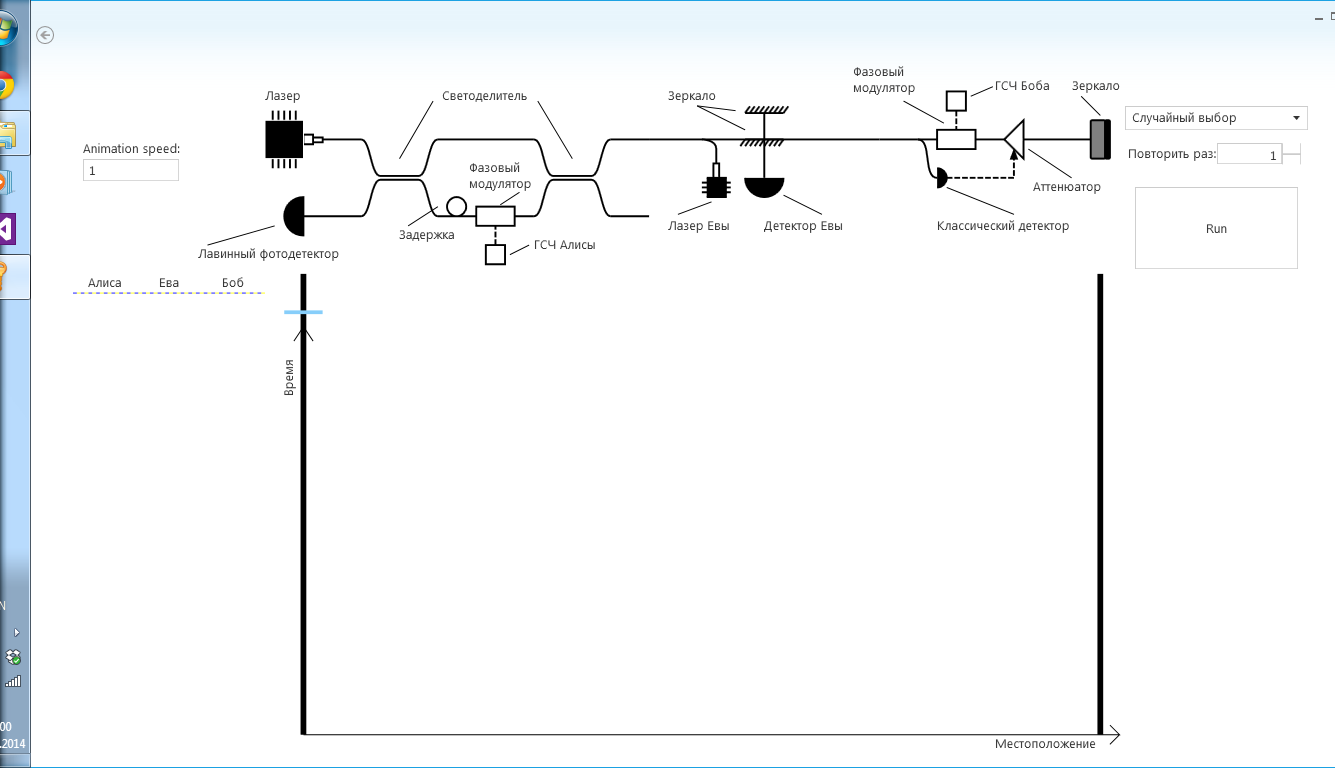
\includegraphics[width=1\linewidth]{screenshots/initial}}
  \caption{Начальное состояние системы}
  \end{figure}
  
  \begin{figure}[h]
  \center{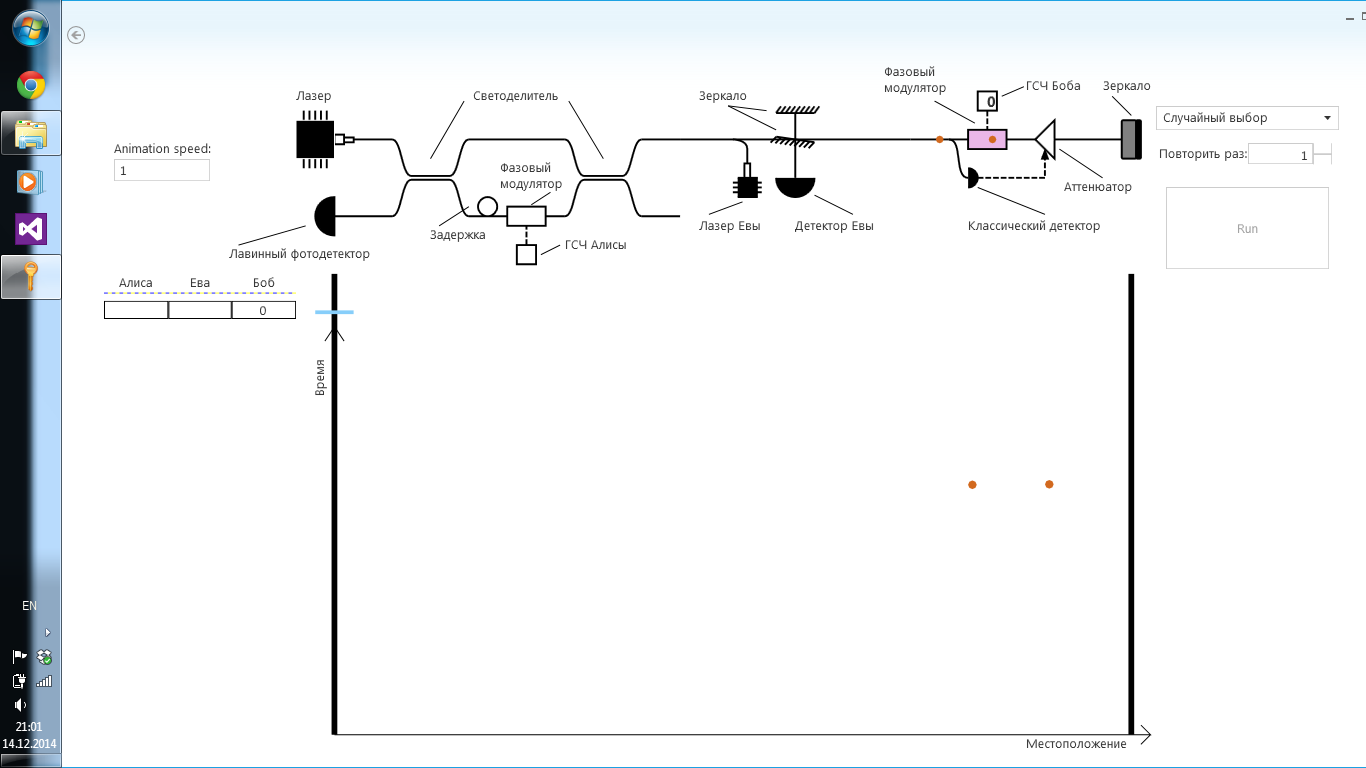
\includegraphics[width=1\linewidth]{screenshots/process}}
  \caption{Система в процессе работы}
  \end{figure}
  
  \begin{figure}[h]
  \center{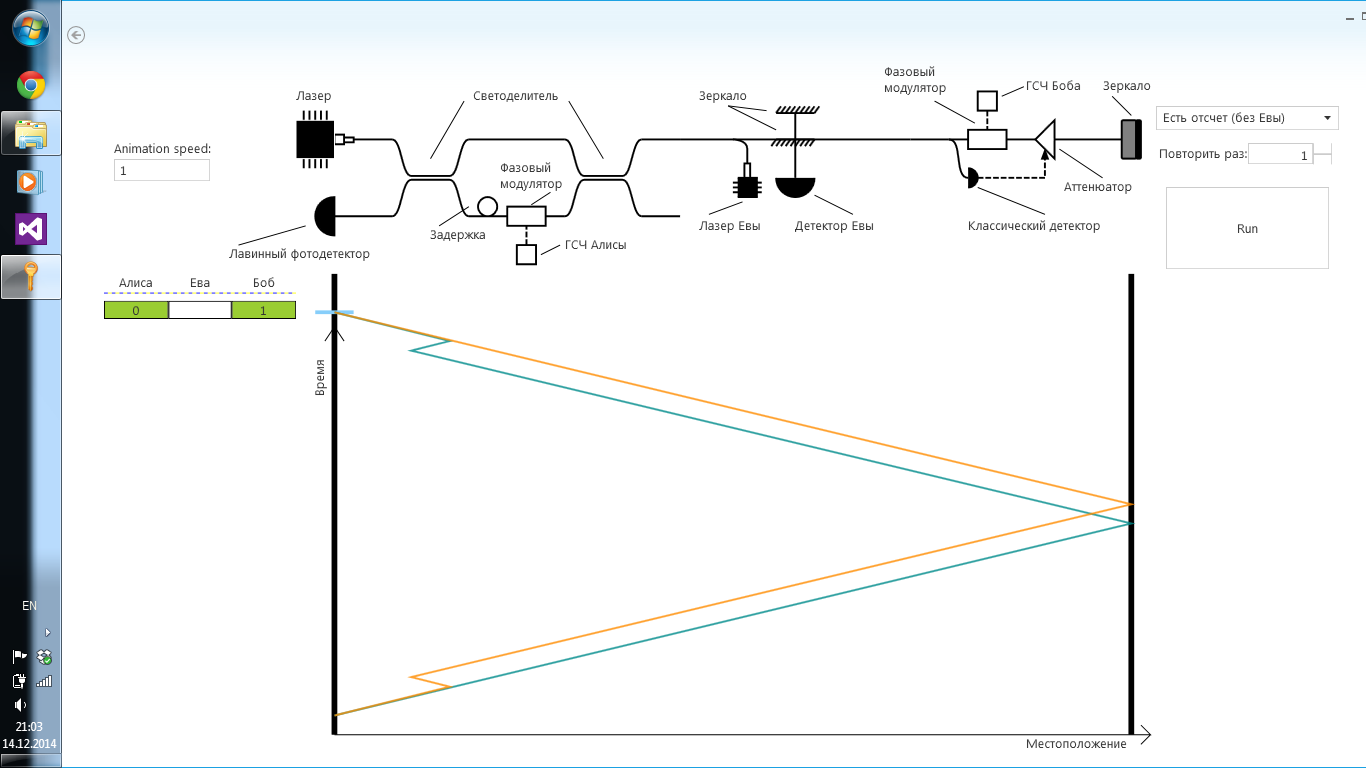
\includegraphics[width=1\linewidth]{screenshots/success}}
  \caption{На этой итерации все прошло успешно и получен еще один бит ключа}
  \end{figure}
  
  \begin{figure}[h]
  \center{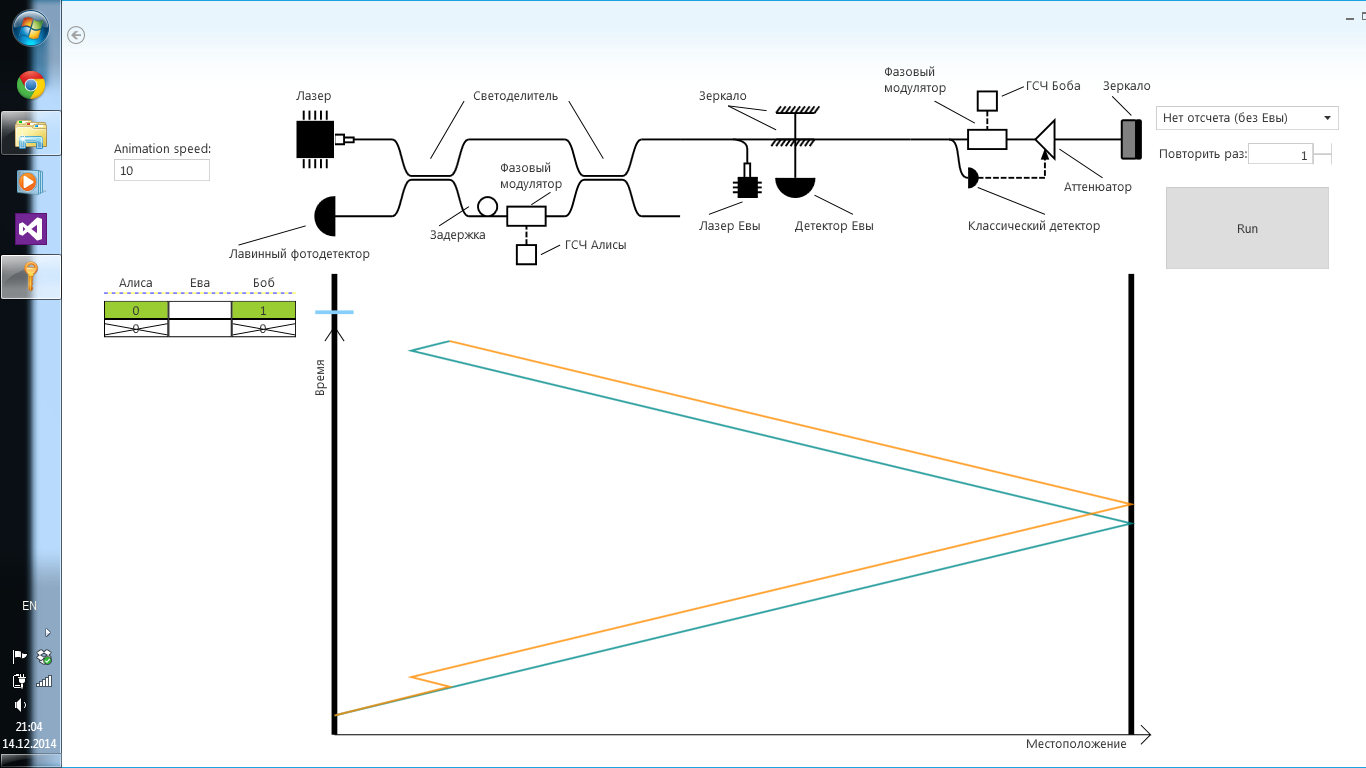
\includegraphics[width=1\linewidth]{screenshots/no_click}}
  \caption{На этой итерации бит ключа получен НЕ будет}
  \end{figure}
  
  \begin{figure}[h]
  \center{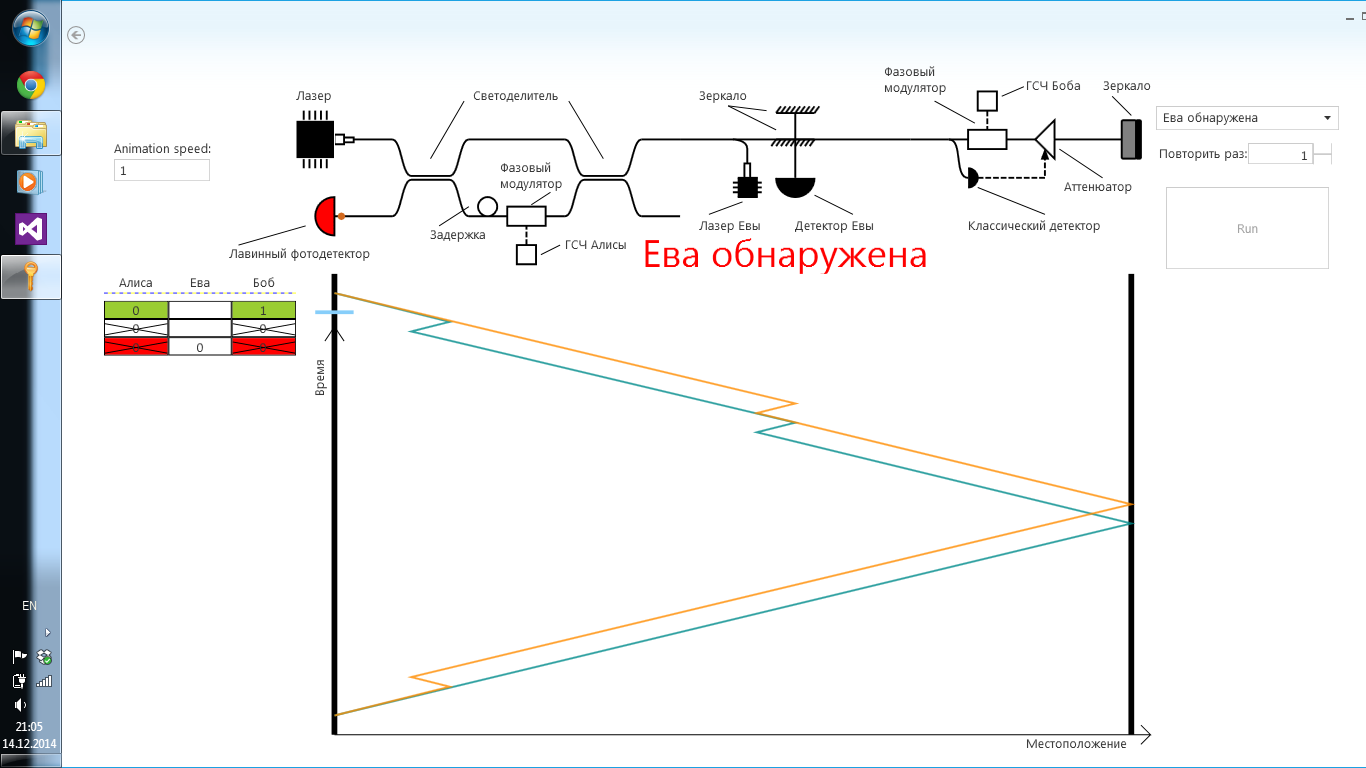
\includegraphics[width=1\linewidth]{screenshots/eva_detected}}
  \caption{Если в канале возникнет злоумышленник, система об этом узнает и предупредит}
  \end{figure}
  
  \begin{figure}[h]
  \center{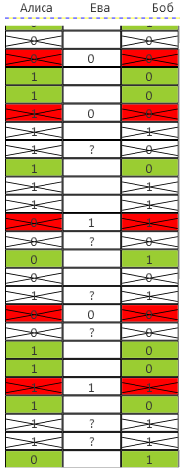
\includegraphics{screenshots/series}}
  \caption{Серия посылок. Из зеленых ячеек в дальнейшем будет получен секретный ключ, остальные посылки будут отброшены}
  \end{figure}


\begin{comment}
Квантовое распределение ключей (QKD)~--- концепт секретного распределения ключей, основанный на фундаментальных законах квантовой механики.
Квантовая криптография \cite{bennett1984QuacryPubkeydiscoitos, ekert1991QuacrybasBelthe, gisin2002Quacry, scarani2009secpraquakeydis, hughes2011Refquacry, lam2013QuacryConimp} приобрела популярность за обещание абсолютной секретности против подслушивания. <<Абсолютной>> понимается в том смысле, что секретность гарантирована
фундаментальными запретами квантовой механики (на копирование неизвестного квантового состояния и невозможности достоверной различимости неортогональных квантовых состояний) \cite{bennett1984QuacryPubkeydiscoitos, bennett1992Quacryusianytwononsta, wootters1982sinquacanbeclo, dieks1982CombyEPRdev}, 
а не нашими технологическими возможностями. Достоверная неразличимость неортогональных квантовых состояний приводит к тому, что любые попытки вторжения в канал связи с целью получения информации о передаваемых состояниях вызывают их неизбежное возмущение, что ведет к ошибкам на приемной стороне и детектированию подслушивателя.
Если ошибка на приемной стороне не превосходит некоторой критической величины\footnote{Величина критической ошибки определяется конкретным протоколом}, то ошибки могут быть исправлены через аутентичный открытый классический канал связи. В результате последующего сжатия (хеширования \cite{bennett1995Genpriamp}) очищенного ключа возникает секретный ключ, известный только двум легитимным пользователям.

Однако, \textit{практические} схемы реализации QKD~--- серьезный вызов для ученых, так как все реализации так или иначе отличаются от теоретических моделей. 
Две основные проблемы всех существующих реализаций, ни одна из которых не может быть эффективно устранена: 
\begin{inparaenum}[\itshape 1\upshape)]
\item любой существующий в настоящее время источник фотонов имеет ненулевую вероятность испустить два или более фотонов одновременно, в то время как в теории нужен ровно один \cite{lounis2000Sinphodemsinmolrootem, benjamin2000Sinphodem}, и
\item наличие потерь в квантовом канале связи.
\end{inparaenum}

В реальной ситуации неоднофотонность источника вместе с потерями в квантовом канале связи приводит к тому, что все базовые протоколы распредения ключей: BB84, B92, SARG04, decoy-state (с состояниями-ловушками), phase-time (фазово-временное кодирование) оказываются неустойчивыми относительно PNS атаки (атака с расщеплением по числу фотонов) и не гарантируют секретность ключей, если длина квантового канала связи превышает некоторую критическую величину. 

Протоколы используются как в оптоволоконных системах квантовой криптографии, так и в системах, работающих через открытое пространство.
Конечной целью работ по квантовой криптографии в открытом пространстве является создание глобальной системы распределения ключей на большие расстояния через низкоорбитальные спутники. 
При передаче ключей через открытое пространство могут быть использованы протоколы, стойкость которых базируется на запретах только квантовой механики, применяемые в оптоволоконных системах квантовой криптографии. 
Однако при не строго однофотонном источнике квантовых состояний и потерях в канале связи дальность передачи секретных ключей при помощи таких протоколов ограничена \cite{scarani2009secpraquakeydis}. 
В принципе можно сформулировать протоколы, дальность которых не ограничена, но при этом неизбежно требуются априорное знание величины потерь и их контроль в канале связи. 
Если для оптоволоконных систем такой подход может оказаться достаточным, то для открытого пространства он неприемлем, посколько априорно потери в канале связи неизвестны и могут меняться в течение передачи ключей. По-видимому, при неоднофотонном источнике и больших априорно не известных потерях, одних только фундаментальных запретов квантовой механики недостаточно для формулировки протоколов, гарантирующих секретность ключей.

Возникает принципиальный и практически важный вопрос о том, существуют ли протоколы квантового распределения ключей, которые обеспечивают безусловную секретность ключей при не строго 
однофотонном источнике и произвольных потерях в квантовом канале связи. Ниже будет предъявлен такой протокол. Данный протокол, кроме ограничений квантовой механики на различимость квантовых состояний, использует дополнительные ограничения, диктуемые специальной теорией относительности.
\end{comment}
\clearpage